\documentclass{scrartcl}

\usepackage{amsmath}
\usepackage{graphicx}
\usepackage[usenames, dvipsnames]{xcolor}

\usepackage{tikz}
\usetikzlibrary{positioning}
\usetikzlibrary{tikzmark}
\usetikzlibrary{calc}

\begin{document}

Bitte dieses Dokument sorgfältig in aller Ruhe durchlesen!  Anschließend die
Aufgaben in jedem Abschnitt machen.

\section{Ableitung = Steigung}

Die Ableitung einer Funktion ist die Steigung an allen Punkten der Kurve der
Funktion.  Die Steigung an einem beliebigen Punkt einer Funktion findet man,
in dem man eine Tangente zu der Kurve der Funktion an diesem Punkt zieht und
dann die Steigung dieser Tangente bestimmt.

Siehe zum Beispiel dieses Diagramm einer quadratischen Funktion.

\includegraphics[width=\textwidth]{quadratic-with-tangents.pdf}

Wenn man einen bestimmten Punkt wählt, dann kann man eine Tangente ziehen an
diesen Punkt.  Diese Tangente ist dann die Ableitung der Funktion \emph{an
diesem Punkt}.  Die allgemeine Form einer Ableitung ergibt eine Funktion,
die besagt, was die Steigung einer Tangente an jedem beliebigen Punkt haben
wird.

\section{Das Ableiten eines Polynoms vom Grad $n$.}
\label{sec:ableiten-grad-n}

Die Ableitung eines Polynoms (z.B. $x^n$) findet man, in dem man die Potenz
als Faktor nimmt, die Potenz des Polynoms um 1 reduziert, und diese
miteinander multipliziert.  Anders gesagt:

\begin{equation}
    x^n \rightarrow n \cdot x^{n-1}
\end{equation}

Hier ist das gleiche Konzept aber anders formuliert:

\begin{equation}
    \text{Sei } f(x) = x^n, \text{dann } f'(x) = n \cdot x^{n-1}
\end{equation}

wo $f'(x)$ ist die Ableitung der Funktion $f(x)$.

\paragraph{Beispiel} Nehmen wir die allgemeine Form einer quadratischen
Funktion:

\begin{equation}
    f(x) = a x^2 + b x + c
\end{equation}

Die Ableitung dieser Funktion ist eine Gerade.  Als Gleichung sieht die
Ableitung so aus:

\begin{equation}
    f'(x) = 2 a x + b
\end{equation}

Der Grund ist, dass die einzelnen Terme so abgeleitet werden:

\begin{align}
    a x^2 & \rightarrow 2 a x\\
    b x & \rightarrow b\\
    c & \rightarrow 0
\end{align}

Betrachten wir den ersten Term genauer.  Hier ist der Prozess des Ableitens
vom ersten Term bildlich dargestellt:

\begin{center}
\resizebox{0.5\textwidth}{!}{
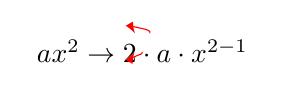
\begin{tikzpicture}[remember picture]
    \node (func) {
        $\tikzmarknode{a1}{a}x^{\tikzmarknode{two1}{2}}
        \rightarrow \tikzmarknode{two2}{2} \cdot
        \tikzmarknode{a2}{a} \cdot x^{2 - 1}$
    };
    \draw[-latex, red] (a1.south) to[out=-60, in=240](a2.south west);
    \draw[-latex, red] (two1.north east) to[out=60, in=120](two2.north west);
\end{tikzpicture}
}
\end{center}

Hier sind die einzelnen Schritte dieses Prozesses.

\begin{align}
    a x^2 & \rightarrow 2 a x^{2 - 1}\\
    & = 2 a x^1\\
    & = 2 a x
\end{align}

Betrachten wir den zweiten Term genauer.  Der Prozess des Ableitens kann
hier auch bildlich dargestellt werden:

\begin{center}
\resizebox{0.5\textwidth}{!}{
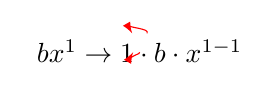
\begin{tikzpicture}[remember picture]
    \node (func) {
        $\tikzmarknode{b1}{b}x^{\tikzmarknode{one1}{1}}
        \rightarrow \tikzmarknode{one2}{1} \cdot
        \tikzmarknode{b2}{b} \cdot x^{1 - 1}$
    };
    \draw[-latex, red] (b1.south) to[out=-60, in=240](b2.south west);
    \draw[-latex, red] (one1.north east) to[out=60, in=120](one2.north west);
\end{tikzpicture}
}
\end{center}

Die einzelnen Schritte dieses Prozesses laufen so:

\begin{align}
    b x = b x^1 & \rightarrow 1 \cdot b x^{1 - 1}\\
    & = 1 \cdot b x^0; \text{ aber } x^0 = 1, \text{deshalb}\\
    & = 1 \cdot b \cdot 1\\
    & = b
\end{align}

\paragraph{Beispiel} Betrachten wir eine spezifische Funktion:

\begin{equation}
    f(x) = 3x^2 - 5x + 2
\end{equation}

Die Ableitung dieser Funktion ist:

\begin{equation}
    f'(x) = 6x - 5
\end{equation}

Der Grund hierfür ist, dass die einzelnen Terme so abgeleitet werden:

\begin{align}
    3x^2 & \rightarrow 6x\\
    -5x & \rightarrow -5\\
    2 & \rightarrow 0
\end{align}

Betrachten wir diesen Prozess genauer, in dem wir jeden Term einzeln
anschauen.  Hier der erste Term:

\begin{align}
    3x^2 & \rightarrow 2 \cdot 3 x^{2 - 1}\\
    & = 6 x^1\\
    & = 6 x
\end{align}

Bildlich dargestellt verläuft der Prozess so:

\begin{center}
\resizebox{0.5\textwidth}{!}{
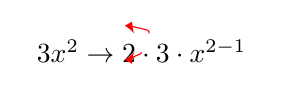
\begin{tikzpicture}[remember picture]
    \node (threex2) {
        $\tikzmarknode{three1}{3}x^{\tikzmarknode{two1}{2}}
        \rightarrow \tikzmarknode{two2}{2} \cdot
        \tikzmarknode{three2}{3} \cdot x^{2 - 1}$
    };
    \draw[-latex, red] (three1.south) to[out=-60, in=240](three2.south west);
    \draw[-latex, red] (two1.north east) to[out=60, in=120](two2.north west);
\end{tikzpicture}
}
\end{center}

Und hier ist der zweite Term:

\begin{align}
    -5x = -5x^1 & \rightarrow 1 \cdot (-5) \cdot x^{1 - 1}\\
    & = 1 \cdot (-5) \cdot x^0; \text{ aber } x^0 = 1, \text{deshalb}\\
    & = 1 \cdot (-5) \cdot 1\\
    & = -5
\end{align}

Wo der Ableitungsprozess auch so dargestellt werden kann:

\begin{center}
\resizebox{0.5\textwidth}{!}{
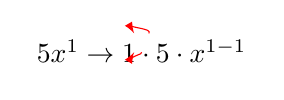
\begin{tikzpicture}[remember picture]
    \node (func) {
        $\tikzmarknode{five1}{5}x^{\tikzmarknode{one1}{1}}
        \rightarrow \tikzmarknode{one2}{1} \cdot
        \tikzmarknode{five2}{5} \cdot x^{1 - 1}$
    };
    \draw[-latex, red] (five1.south) to[out=-60, in=240](five2.south west);
    \draw[-latex, red] (one1.north east) to[out=60, in=120](one2.north west);
\end{tikzpicture}
}
\end{center}

\section{Ableitung einer Konstante}
\label{sec:ableitung-konstante}

Die Ableitung einer Konstante ist 0 (Null), da die Steigung einer Kurve mit
konstantem Wert Null ist.

Zum Beispiel, schaue dieses Diagramm der Funktion $f(x) = 3$ an:

\includegraphics[width=\textwidth]{constant-function.pdf}

Siehe, das die Funktion keine Steigung hat. Das bedeutet, dass die Ableitung
dieser Funktion gleich 0 (Null) ist.

\subsection{Aufgaben}
\label{ex:constants}

Finde die Ableitung der folgenden Funktionen:

\begin{enumerate}
    \item $f(x) = 3$
    \item $f(x) = -5$
    \item $f(x) = \frac{1}{2}$
    \item $f(x) = 6 - 2$
\end{enumerate}

\section{Ableitung einer Gerade}
\label{sec:ableitung-gerade}

Die Ableitung einer Gerade ist die Steigung der Kurve der Gerade.  Die
allgemeine Form einer Funktion, die eine Gerade darstellt ist:

\begin{equation}
    f(x) = m x + b
\end{equation}

wobei $m$ die Steigung der Kurve ist und $b$ is der Schnittpunkt der Gerade
mit der $y$-Achse.

\begin{center}
\resizebox{1\textwidth}{!}{
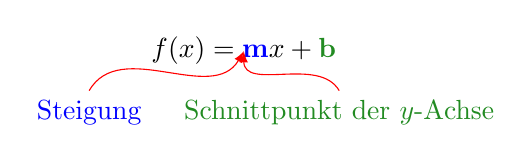
\begin{tikzpicture}[remember picture]
    \node (func) {
        $f(x) = \tikzmarknode{m}{\textcolor{blue}{\textbf{m}}} x +
        \tikzmarknode{b}{\textcolor{ForestGreen}{\textbf{b}}}$
    };
    \node[anchor=north east] (steigung) at ($(m.south west) - (1, 0.5)$)
    {\textcolor{blue}{Steigung}};
    \node[anchor=north west] (schnitt) at ($(b.south east) - (1, 0.5)$)
    {\textcolor{ForestGreen}{Schnittpunkt der $y$-Achse}};
    \draw[-latex, red] (steigung.north) to[out=60, in=240](m.south);
    \draw[-latex, red] (schnitt.north) to[out=120, in=270](b.south);
\end{tikzpicture}
}
\end{center}

Da die Steigung der Funktion $f(x)$ durch den Koeffizienten $m$ dargestellt
wird, kann man sehen, dass die Ableitung gleich $m$ ist.  Anders gesagt, die
Ableitung von $f(x)$ ist:

\begin{equation}
    f'(x) = m
\end{equation}

\paragraph{Beispiel} Betrachten wir als spezifisches Beispiel die folgende
Funktion:

\begin{equation}
    f(x) = 10 x - 2
\end{equation}

Diese Funktion hat die allgemeine Form einer Gerade wie oben erwähnt, siehe:

\begin{align}
    f(x) = & 10 x - 2\\
    \text{Form: } & m x + b
\end{align}

Wo $m$ (die Steigung der Gerade) entspricht den Wert 10 und $b$ (der
Schnittpunkt der $y$-Achse) entspricht den Wert $-2$.

Da die Steigung der Gerade den Wert 10 hat, können wir direkt sagen, dass
die Ableitung von $f(x)$ ist:

\begin{equation}
    f'(x) = 10
\end{equation}

Wir können dies auch sehen anhand der Diskussion über das Ableiten eines
Polynoms vom Grad $n$ im Abschnitt~\ref{sec:ableiten-grad-n}:

\begin{align}
    f(x) &\rightarrow f'(x)\\
    10 x - 2 = 10 \cdot x^1 - 2 &\rightarrow 10 \cdot x^{1 - 1} - 0\\
    &= 10 \cdot x^0; \text{wobei } x^0 = 1, \text{deshalb}\\
    &= 10 \cdot 1\\
    &= 10
\end{align}

Was heißt, dass die Ableitung so geschrieben werden kann:

\begin{equation}
    f'(x) = 10
\end{equation}

\paragraph{Beispiel} Betrachten wir ein weiteres Beispiel:

\begin{equation}
    f(x) = -12 x + 9
\end{equation}

Wieder sehen wir, dass die Funktion der allgemeinen Form der Funktion einer
Gerade entspricht:

\begin{alignat}{3}
    f(x) = && -12 x &&+ 9\\
    \text{Form: } && m x &&+ b
\end{alignat}

Da $m$ die Steigung der Gerade ist, was den Wert $-12$ entspricht, kann man
direkt sagen, dass die Ableitung von $f(x)$ ist:

\begin{equation}
    f'(x) = -12
\end{equation}

Und ja, man kann eine negative Steigung haben!  Das heißt nur, dass die
Kurve nach unten zeigt.  Wenn die Steigung positiv ist, dann zeigt die Kurve
nach oben.

Wenn wir den allgemeinen Prozess für die Ableitung eines Polynoms benutzen
(wie aus der Diskussion in Abschnitt~\ref{sec:ableitung-grad-n}), dann
bekommen wir dasselbe Ergebnis.  Schau:

\begin{align}
    f(x) &\rightarrow f'(x)\\
    -12x + 9 &\rightarrow -12 \cdot x^{1 - 1} - 0\\
    &= -12 \cdot x^0; \text{wobei } x^0 = 1, \text{deshalb}\\
    &= -12 \cdot 1\\
    &= -12
\end{align}

Damit kann man die Ableitung der Funktion $f(x)$ so schreiben:

\begin{equation}
    f'(x) = -12
\end{equation}

\subsection{Aufgaben}
\label{ex:straight-lines}

Finde die Ableitung der folgenden Funktionen:

\begin{enumerate}
    \item $f(x) = 10 x - 2$
    \item $f(x) = 2 x - 1$
    \item $f(x) = 14 x + 19$
    \item $f(x) = -12 x + 9$
\end{enumerate}

\section{Ableitung einer quadratischen Funktion}

Eine quadratische Funktion hat die folgende allgemeine Form:

\begin{equation}
    f(x) = ax^2 + bx + c
\end{equation}

Wie in Abschnitt~\ref{sec:ableiten-grad-n} diskutiert, ist die Ableitung
einer quadratischen Funktion eine Gerade.  Die Ableitung von $f(x)$ ist:

\begin{equation}
    f'(x) = 2ax + b
\end{equation}

Setzen wir den Koeffizienten $2a$ gleich $m$, d.h.:

\begin{equation}
    m = 2 \cdot a
\end{equation}

dann können wir die Ableitung oben so schreiben:

\begin{equation}
    f'(x) = mx + b
\end{equation}

was die allgemeine Form einer Gerade entspricht.

\paragraph{Beispiel} Betrachten wir eine spezifische quadratische Funktion:

\begin{equation}
    f(x) = 7 x^2 + 19 x - 6
\end{equation}

Um die Ableitung von $f(x)$ zu finden, können wir die Ableitung von jedem
einzelnen Term finden und kombinieren.  Die Ableitung des ersten Terms ist:

\begin{align}
    7 x^2 &\rightarrow 7 \cdot 2 \cdot x^{2 - 1}\\
    &\rightarrow 7 \cdot 2 \cdot x^1\\
    &\rightarrow 7 \cdot 2 \cdot x\\
    &\rightarrow 14 x
\end{align}

Die Ableitung des zweiten Terms ist wie folgt.

\begin{quotation}
\textbf{Merke:} dieser Term ist \emph{linear} in $x$, was heißt, dass er wie
eine Gerade wirkt und deshalb kann man diesen Term wie eine Gerade Funktion
ableiten wie in Abschnitt~\ref{sec:ableitung-gerade} diskutiert.
\end{quotation}

\begin{align}
    19 x = 19 x^1 &\rightarrow 19 \cdot 1 \cdot x^{1 - 1}\\
    &= 19 \cdot 1 \cdot x^0; \text{wobei } x^0 = 1, \text{deshalb}\\
    &= 19 \cdot 1 \cdot 1\\
    &= 19
\end{align}

Der letzte Term ist eine Konstante, deshalb können wir diesen Term wie
Konstanten ableiten, wie im Abschnitt~\ref{sec:ableitung-konstante}
diskutiert.  Das heißt, dass die Ableitung dieses Terms ist 0 (Null):

\begin{equation}
    -6 \rightarrow 0
\end{equation}

Wir kombinieren jetzt die Ableitung des ersten Terms ($14x$) mit der
Ableitung des zweiten Terms ($19$) und der Ableitung des letzten Terms
($0$), um die Ableitung der ursprünglichen Funktion zu bestimmen:

\begin{equation}
    f'(x) = 14 x + 19
\end{equation}

\subsection{Aufgaben}
\label{ex:quadratics}

Finde die Ableitung der folgenden Funktionen:

\begin{enumerate}
    \item $f(x) = x^2 - x - 12$
    \item $f(x) = -x^2 + 14x + 40$
    \item $f(x) = 3x^2 - 2x - 8$
    \item $f(x) = \frac{3}{2}x^2 - 5x$
    \item $f(x) = 7x^2 + 19x - 6$
\end{enumerate}

\newpage

\section{Lösungen}

\subsection*{Ableitung einer Konstante (Aufgaben~\ref{ex:constants})}

\begin{enumerate}
    \item 0
    \item 0
    \item 0
    \item 0
\end{enumerate}

Das ist kein Witz: alle Antworten sind 0 (Null), da die Ableitung einer
Konstante immer Null ist.

\subsection*{Ableitung einer Gerade (Aufgaben~\ref{ex:straight-lines})}

\begin{enumerate}
    \item 10
    \item 2
    \item 14
    \item -$12$
\end{enumerate}

\subsection*{Ableitung einer quadratischen Funktion (Aufgaben~\ref{ex:quadratics})}

\begin{enumerate}
    \item $2x - 1$
    \item $-2x + 14$
    \item $6x - 2$
    \item $3x - 5$
    \item $14x + 19$
\end{enumerate}

\end{document}
